\section{Subgradient Methods}

\textbf{Separating plane of two convex sets}: let $S$ and $T$ be two nonempty convex sets. A hyperplane $a^\top x = b$ is said to separate $S$ and $T$ if $S \cup T \not\subset H$, $S \subset H^-=\{x: a^\top x \le b\}$ and $T \subset H^+ = \{x: a^\top x \ge b\}$. If further $S \subset H^{--}=\{x: a^\top x < b\}$ and $T \subset H^{++} = \{x: a^\top x > b\}$, then $H$ is said to strictly separate $S$ and $T$.

\textbf{Hyperplane separation theorem}: for two non-empty convex sets $S$ and $T$, they can be separated by a hyperplane iff $\rint(S) \cap \rint(T) = \emptyset$.

\textbf{Definitions}:
\begin{enumerate}
    \item \textbf{Subgradient}: let $f$ be a convex function, then a vector $g$ is a subgradient of $f$ at $x$ if $f(y) \ge f(x) + g^\top (y-x)$.
    \item \textbf{Subdifferential}: the set of all subgradient at $x$ is called the subdifferential of $f$ at $x$, denoted as $\partial f$.
    \item \textbf{Directional derivative}: the directional derivative of $f$ at $x$ along $d$ is $f^\prime(x;d) = \lim_{\delta \rightarrow 0^+} \frac{f(x+\delta d) - f(x)}{\delta}$.
\end{enumerate}

\textbf{Properties}:
\begin{enumerate}
    \item \textbf{subgradient = gradient, when convex and differentiable}: (6.2) if $f$ is convex and differentiable at $x$, then $\partial f=\{\nabla f(x)\}$; (6.3) if $f$ is only differentiable but not convex, then $\partial f \subseteq \{\nabla f(x)\}$. Proof: clearly $\{\nabla f(x)\} \subseteq \partial f$ given $f$ convex; assume $\partial f \ne \emptyset$, let $y = x+\epsilon d$ for small $\epsilon$, then $\frac{f(y) - f(x)}{\epsilon} \ge g^\top d$, which means $\nabla f(x)^\top d \ge g^\top d$ for any $d$. This implies $g = \nabla f(x)$.
    \item \textbf{Bounded subgradient for convex functions = Lipschitz}: (6.5) if $f$ is convex and $\dom(f)$ is open, then $\|g\| \le B$ for all $x$ and $g \in \partial f(x)$ is equivalent to $|f(x)-f(y)| \le B \|x-y\|$ for all $x,y$. Proof: (i) one side: let $y=x+\epsilon g$ for some $\epsilon >0$. Then $f(y)-f(x) \ge \epsilon \|g\|^2$. By $B$-Lipschitz, $f(y) -f(x) \le B\|y-x\| = \epsilon B \|g\|$. These two imply $\|g\|\le B$. (ii) the other side: for any $x,y$ and $g \in \partial f(x)$, $f(x) - f(y) \le g^\top (x-y) \le \|g\|\|x-y\| \le B\|x-y\|$ and $f(y) - f(x) \ge g^\top (y-x) \ge -B \|y-x\|$.
    \item \textbf{Convexity means subgradient almost everywhere}: (6.10) let $f$ be convex and $x \in \rint(\dom(f))$, then $\partial f(x)$ is non-empty and bounded. Proof: (i) non-emptiness: w.l.o.g, assume $\dom(f)$ is full-dimensional and $x \in \text{int}(\dom(f))$. Since $\epi(f)$ is convex, by hyperplane separation theorem, $\exists s, \beta$, s.t. $s^\top y + \beta t \ge s^\top x + \beta f(x)$ for any $(y,t) \in \epi(f)$. Since $t$ can be arbitratily large, we have $\beta \ge 0$. If $\beta = 0$, then $s^\top (y-x) \ge 0$ for any $y$, which means $s=0$, a contradiction. Thus, $\beta > 0$. Setting $g = -\beta^{-1} s$, we get $f(y) \ge f(x) + g^\top (y-x)$. (ii) boundness: suppose $\exists g_k \in \partial f(x)$ s.t. $\|g_k\| \rightarrow +\infty$. Since $x\in\text{int}(\dom(f))$, $\exists \delta>0$, s.t. $B(x, \delta) \subseteq \dom(f)$. Therefore, $y_k := x+\delta \frac{g_k}{\|g_k\|} \in \dom(f)$. By definition, $f(y_k) \ge f(x) + g_k^\top (y_k - x) = f(x) + \delta \|g_k\| \rightarrow +\infty$, a contradition.
    \item \textbf{Subgradient everywhere means convexity}: if $\dom(f)$ is convex and for any $x \in \dom(f)$, $\partial f(x)$ is non-empty, then $f$ is convex. Proof: for any $x, y \in \dom(f)$ and $\lambda \in (0,1)$, let $z = \lambda x + (1-\lambda) y$ and $g \in \partial f(z)$. Then $f(x) \ge f(z) + g^\top (x-z)$ and $f(y) \ge f(z) + g^\top (y-z)$. Adding them leads to definition of convexity.
    \item \textbf{$\text{dist}(0, \partial f(x))$ decides optimality}: if $0 \in \partial f(x)$, then $x$ is a global minimum. Proof: by definition.
    \item \textbf{Subgradient and directional derivative}: (6.13) let $f$ be convex and $x \in \text{int}(\dom(f)),$ then $f^\prime(x ;d) = \max_{g \in \partial f(x)} g^\top d$. Proof: by the definition of subgradient. we have $f(x+\delta d) - f(x) \ge \delta g^\top d$, which implies $f^\prime(x ; d) \ge g^\top d$ for any $g \in \partial f(x)$ and thus $f^\prime(x ; d) \ge \max_{g \in \partial f(x)} g^\top d$. To conclude the other side, consider $C_1 = \{(y,t): f(y)<t\}$ and $C_2 = \{(y,t): y=x+\alpha d, t = f(x)+\alpha f^\prime(x;d), \alpha \ge 0\}$. Clearly they are convex and non-empty. If $C_1 \cap C_2 = \emptyset$, then by hyperplane separation theorem, $\exists g_0, \beta$, s.t. $g_0^\top (x+\alpha d) + \beta (f(x) + \alpha f^\prime(x;d)) \le g_0^\top y + \beta t$ for any $\alpha \ge 0$ and any $t > f(y)$. Similar to the proof of (6.10), we can show $\beta > 0$. Let $\tilde{g}=\beta^{-1} g_0$, we have $\tilde{g}^\top (x+\alpha d) + f(x) + \alpha f^\prime(x;d) \le \tilde{g}^\top y + f(y)$ . Set $\alpha = 0$, we have $\tilde{g}x + f(x) \le \tilde{g}^\top y + f(y)$, which means $-\tilde{g} \in \partial f(x)$. Further, set $y=x$ and $\alpha=1$, we have $f^\prime(x;d) \le - \tilde{g}^\top d \le \max_{g \in \partial f(x)} g^\top d$.
\end{enumerate}

\textbf{Calculus of subgradient}:
\begin{enumerate}
    \item For $h(x) = \lambda f(x) + \mu g(x)$ where $\lambda, \mu \ge 0$ and $f,g$ both are convex, then $\partial h(x) = \lambda \partial f(x) + \mu \partial g(x)$.
    \item For $h(x) = f(Ax+b)$ where $f$ is convex, then $\partial h(x) = A^\top \partial f(Ax+b)$.
    \item For $h(x) = \sup_{\alpha \in A} f_\alpha(x)$ and each $f_\alpha(x)$ is convex, then $\partial h(x) \supseteq \text{conv}\{\partial f_\alpha(x): f_\alpha(x) = h(x)\}$.
    \item For $h(x) = F(f_1(x), \dots, f_m(x))$ where $F$ is non-decreasing and convex, then $\partial h(x) \supseteq \{\sum_{i=1}^m d_i \partial f_i(x): (d_1, \dots, d_m) \in \partial F(y_1, \dots, y_m)\}$.
\end{enumerate}

\subsection{Subgradient descent} 
Consider $f$ convex (possibly non-differentiable) on a closed and convex set $X$. The subgradient descent does $x_{t+1} = \Pi_X(x_t - \gamma_t g(x_t))$, where $g(x_t) \in \partial f(x_t)$. When $f$ is differentiable, this reduces to PGD. However, moving towards the negative direction of subgradient is not necessarily decreasing the objective. Therefore, we can only measure $\min_{t \le T} f(x_t) - f^*$ instead of $f(x_T)-f^*$.

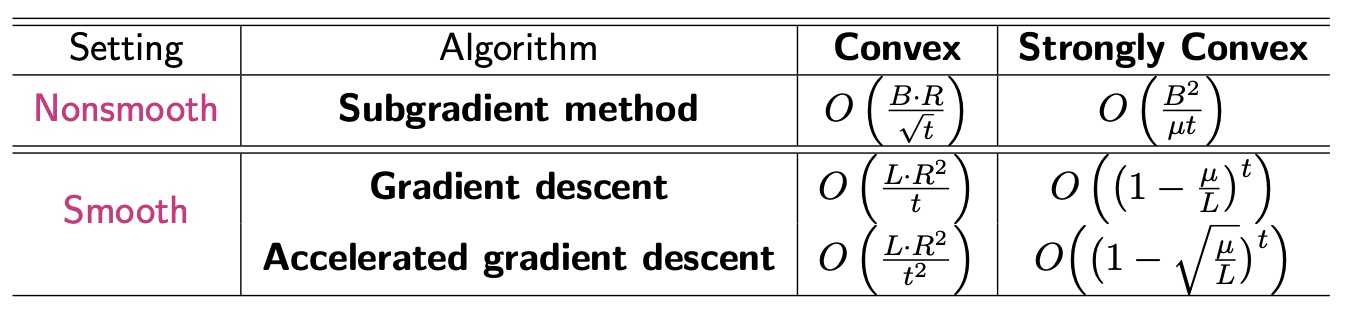
\includegraphics[width=\linewidth]{imgs/subGD.jpg}

\textbf{Analysis for convex functions}:
\begin{enumerate}
    \item \textbf{General analysis}: (6.17) starting from $x_1$, we have $\min_{1\le t\le T} f(x_t) - f^* \le \frac{1}{2}(\sum_{t=1}^T \gamma_t)^{-1}(\|x_1 - x^*\|^2 + \sum_{t=1}^T \gamma_t^2\|g(x_t)\|^2)$ and $f(\hat{x}_T) - f^* \le \frac{1}{2}(\sum_{t=1}^T \gamma_t)^{-1}(\|x_1 - x^*\|^2 + \sum_{t=1}^T \gamma_t^2\|g(x_t)\|^2)$ for $\hat{x}_t=(\sum_{t=1}^T \gamma_t)^{-1}(\sum_{t=1}^T \gamma_t x_t)$. Proof: by definition, $\|x_{t+1} - x^*\|^2 = \|\Pi_X(x_t - \gamma_t g(x_t)) - x^*\|^2 \le \|x_t - \gamma_t g(x_t) - x^*\|^2 = \|x_t - x^*\|^2 - 2\gamma_t g(x_t)^\top (x_t - x^*) + \gamma_t^2\|g(x_t)\|^2$. By definition of subgradient, we have $f(x_t) - f^* \le g^\top (x_t - x^*)$. These two gives $\sum_{t=1}^T \gamma_t (f(x_t) - f^*) \le \frac{1}{2}(\|x_1 - x^*\|^2 - \|x_{T+1} - x^*\|^2 + \sum_{t=1}^T \gamma_t^2\|g(x_t)\|^2) \le \frac{1}{2}(\|x_1 - x^*\|^2 + \sum_{t=1}^T \gamma_t^2\|g(x_t)\|^2)$. In addition, we have $\min_{t} f(x_t) - f^* \le (\sum_{t=1}^T \gamma_t)^{-1} (\sum_t \gamma_t (f(x_t) - f^*))$, thus the first claim follows. For the second claim, use $\sum_t \gamma_t (f(x_t) - f^*) \ge (\sum_t \gamma_t) (f(\hat{x}_t) - f^*)$ by convexity.
    \item \textbf{Lipschitz functions}: assume $\|x_1 - x^*\| \le R$ and $\|g(x_t)\| \le B$, then $\min f(x_t) - f^* \le \frac{1}{2}(\sum_{t=1}^T \gamma_t)^{-1} (R^2 + \sum_t \gamma_t^2 B^2)$.
\end{enumerate}

\textbf{$O(1/\sqrt{t})$ convergence under different stepsizes for  convex Lipschitz functions}:
\begin{enumerate}
    \item $\gamma_t = \gamma$: $\epsilon_t = \frac{1}{2}(\frac{R^2}{T\gamma} + B^2\gamma) \rightarrow \frac{B^2}{2}\gamma$. Choose $\gamma_t = \frac{R}{B\sqrt{T}}$, we have $\epsilon_t \le \frac{RB}{\sqrt{T}}$.
    \item $\sum_t \gamma_t \rightarrow +\infty$ and $\gamma_t \rightarrow 0$: we have $\epsilon_t \rightarrow 0$. If set $\gamma_t = \frac{R}{B\sqrt{t}}$, we get $\epsilon_t = O(\frac{BR}{\sqrt{T}})$
    \item $\sum_t \gamma_t \rightarrow +\infty$ and $\sum_t \gamma_t^2 < +\infty$: $\epsilon_t \rightarrow 0$.
    \item Polyak stepsize $\gamma_t = \frac{f(x_t) - f^*}{\|g(x_t)\|^2}$: this makes the general analysis to give $\|x_{t+1} - x^*\|^2 \le \|x_t - x^*\|^2 - 2\gamma_t g(x_t)^\top (x_t - x^*) + \gamma_t^2 \|g(x_t)\|^2 \le \|x_t - x^*\|^2 - 2\gamma_t (f(x_t) - f^*) + \gamma_t^2 \|g(x_t)\|^2 = \|x_t - x^*\|^2 - \frac{(f(x_t) - f^*)^2}{\|g(x_t)\|^2} \le  \|x_t - x^*\|^2 - \frac{(f(x_t) - f^*)^2}{B^2}$, thus guarantees the decrease of $\|x_t - x^*\|$. This implies $\sum_t (f(x_t) - f^*)^2 \le R^2 B^2$, thus $\epsilon_t = O(\frac{RB}{\sqrt{T}})$.
\end{enumerate}

\textbf{$O(1/t)$ convergence for strongly convex Lipschitz functions}:
\begin{enumerate}
    \item (6.18) Let $f$ be $\mu$-strongly convex. With $\gamma_t = \frac{1}{\mu t}$, we have $\min f(x_t) - f^* \le \frac{B^2(\log(T)+1)}{2\mu T}$ and $f(\hat{x}_T) - f^* \le \frac{B^2(\log(T)+1)}{2\mu T}$ for $\hat{x}_T = \frac{1}{T}\sum_t x_t$. Proof: by strong convexity, $f(y) - f(x) + g(x)^\top (y-x) + \frac{\mu}{2}\|y-x\|^2$. Thus, general analysis gives $\|x_{t+1} - x^*\|^2 \le \|x_t-x^*\|^2 - 2\gamma_t (f(x_t) - f^* + \frac{\mu}{2}\|x_t - x^*\|^2) + \gamma_t^2 \|g(x_t)\|^2$, which implies an upper bound on $f(x_t) - f^*$. Following the same steps in the general analysis, we get the desired result.
    \item (6.19) Let $f$ be $\mu$-strongly convex. With $\gamma_t = \frac{2}{\mu (t+1)}$, we have $\min f(x_t) - f^* \le \frac{2B^2}{\mu (T+1)}$ and $f(\hat{x}_T) - f^* \le \frac{2B^2}{\mu (T+1)}$ for $\hat{x}_T = \sum_t \frac{2t}{T(T+1)} x_t$. Proof: the same analysis gives $t(f(x_t) - f^*) \le \frac{\mu t(t-1)}{4}\|x_t - x^*\|^2 - \frac{\mu t (t+1)}{4}\|x_{t+1}-x^*\|^2 + \frac{B^2}{\mu (t+1)}$. The result follows.
\end{enumerate}

\textbf{Subgradient descent is asymptotically optimal for first-order subgradient methods}: (Thm 6.20): for any $1\le t \le n$ and $x_1 \in \mathbb{R}^n$, there exists a $B$-Lipschitz continuous function $f$ and a convex set $X$ with diameter $R$, s.t. for any first-order method that generates $x_t \in x_1 + \text{span}(g(x_1), \dots, g(x_{t-1}))$, where $g(x_i) \in \partial f(x_i)$, we have $\min_{1\le s\le t}f(x_s) - f^* \ge \frac{BR}{4(1+\sqrt{t})}$. In addition, there exists a $B$-Lipschitz continuous function $f$ that is $\mu$-strongly convex, s.t. $\min_{1\le s\le t}f(x_s) - f^* \ge \frac{B^2}{8\mu t}$. Proof: W.l.o.g., assume $x_1=0$. Let $X = \{x:\|x\| \le R/2\}$ and $f(x) =  C\max_{1\le i\le t}x_i + \frac{\mu}{2}\|x\|^2$ for some $C>0, \mu >0$. The subgradient of $f$ is $\partial f(x) = \mu x + C \cdot \text{conv}\{e_i: i \text{ s.t. } x_i=\max_{1\le j \le t}x_j\}$. The optima of $f$ is $f^* = - \frac{C^2}{2\mu t}$. Consider $g(x)=Ce_i+\mu x$, where $i$ is the first coordinate that $x_i = \max_{1\le j \le t} x_j$. Since the algorithm runs for $t$ iterations, the last dimension cannot be updated. Therefore, $\min_{1\le s \le t}f(x_s) - f^* \ge \frac{C^2}{2\mu t}$. (1) Let $C = \frac{B\sqrt{t}}{1+\sqrt{t}}$ and $\mu = \frac{2B}{R(1+\sqrt{t})}$, we have $\max_{g \in \partial f(x)}\|g\| \le C + \mu \|x\|\le R$, and the first result follows. (2) Let $C=\frac{B}{2}$ and $\mu = \frac{B}{R}$, we have $\max_{g \in \partial f(x)}\|g\| \le C + \mu \|x\|\le R$, $f$ is $\mu$-strongly convex, and the second result follows.

\subsection{Mirror Descent}

Mirror descent only uses subgradients, and have the same aymptotic performance as subgradient descent. However, it may have better constants than subgradient descent. Subgradient descent is a special case of mirror descent.

\textbf{Definitions}:
\begin{enumerate}
    \item \textbf{Bregman Divergence}: let $w(x)$ be strictly convex and continuously differentiable on a close convex $X$. $V_w(x, y) = w(x) - w(y) - \nabla w(y)^T (x-y)$ is defined to be the Bregman divergence. This is asymmetric, thus not a valid distance. If $w$ is $\mu$-strongly convex, then $V_w(x, y)$ is $\mu$-strongly convex in $x$.
    \item \textbf{Prox-mapping}: given an input $x$ and vector $\xi$, the prox-mapping is defined as $\Prox_x(\xi) = \argmin_{u\in X}\{V_w(u, x) + \langle \xi, u \rangle\}$, where $w$ is $1$-strongly convex. 
    \item \textbf{Mirror Descent}: do $x_{t+1} = \Prox_{x_t}(\gamma_t g(x_t)) = \argmin_{x\in X}\{w(x)+\langle \gamma_t g(x_t)-\nabla w(x_t), x\rangle\}$. Recall that the subgradient descent is equivalent to $x_{t+1}=\argmin_{x \in X} \{\frac{1}{2}\|x-x_t\|^2 + \langle \gamma_t g(x_t), x\rangle\}$ and $V_w(x,y)=\frac{1}{2}\|x-y\|^2$ for $w(x) = \frac{1}{2}\|x\|^2$. Therefore, subgradient descent is a special case of mirror descent.
\end{enumerate}

\textbf{Properties}:
\begin{enumerate}
    \item \textbf{Three point identity}: (6.26) $V_w(x, z) = V_w(x, y) + V_w(y, z) - \langle \nabla w(z) - \nabla w(y), x-y \rangle$. Proof: by definition.
    \item \textbf{Generalized Pythagorean Theorem for Bregman Divergence}: (6.23) if $x^* = \argmin_{x \in C} V_w(x, x_0)$ for some convex set $C$, then for any $y \in C$, we have $V_w(y, x_0) \ge V_w(y, x^*) + V_w(x^*, x_0)$. Proof: use $\nabla V_w(x, x_0)^\top \mid_{x=x^*} (y-x^*) \ge 0 \Leftrightarrow (\nabla w(x^*) - \nabla w(x_0))^\top (y-x^*) \ge 0$ and the three point identity.
    \item \textbf{Convergence of mirror descent}: (6.28) let $f$ be convex, we have $\min_{1 \le t \le T}f(x_t) - f^* \le \frac{1}{\sum_{t=1}^T \gamma_t} (V_w(x^*, x_1) + \frac{1}{2}\sum_{t=1}^T \gamma_t^2 \|g(x_t)\|^2)$. Proof: since $x_{t+1} =  \argmin_{x\in X}\{w(x)+\langle \gamma_t g(x_t)-\nabla w(x_t), x\rangle\}$, by optimality we have $\langle \nabla w(x_{t+1}) + \gamma_t g(x_t) - \nabla w(x_t), x-x_{t+1}\rangle \ge 0$. Therefore, we have $\langle \gamma_t g(x_t), x_{t+1} -x \rangle \le \langle \nabla w(x_{t+1}) - \nabla w(x_t), x-x_{t+1} \rangle = V_w(x, x_t) - V_w(x, x_{t+1}) - V_w(x_{t+1}, x_t)$. Using $\langle \gamma_t g(x_t), x_t - x_{t+1}\rangle \le \frac{\gamma_t^2}{2}\|g(x_t)\|^2 + \frac{1}{2}\|x_t - x_{t+1}\|^2$ and noticing $V_w(x_{t+1}, x_t) \ge \frac{1}{2}\|x_t - x_{t+1}\|^2$ by 1-strongly convexity, we have $\langle \gamma_t g(x_t), x_t - x^* \rangle \le V_w(x^*, x_t) - V_w(x^*, x_{t+1}) + \frac{\gamma_t^2}{2}\|g(x_t)\|^2$. The rest is the same as the proof of (6.17).
\end{enumerate}
